\section{Experiments and Results}
\label{sec:experiments}

We evaluate our neuron population reconstruction approach in a large-scale OM image slice of a mouse brain in dimension of $25397\times 18516\times 869$ ($761$GB), as Fig.~\ref{fig:brain} shows.
%
The image \md{is} captured by the VISoR imaging system~\cite{Wang2019} at a physical resolution of $0.5 \times0.5 \times 0.5$ \SI{}{\micro\metre}$^3$ per voxel. 
%
The image intensity is in 16-bit dynamic range, which preserves sufficient signal details.
In order to evaluate our PLNPR method for neuronal reconstruction in local blocks, we first conduct extensive experiments on the VISoR-40 dataset which we build and the BigNeuron dataset~\cite{peng2015}. 
%
Then we test our UltraNPR algorithm for neuronal population reconstruction in a slice of the mouse brain image.

\subsection{Evaluation of PLNPR on VISoR-40 Dataset}
\label{sec:exp_PLNPR_VISoR}

\subsubsection{VISoR-40 Dataset}
Though many neuron tracing techniques have been proposed, there is no dataset of OM images for dense neuronal population reconstruction.
We construct a neuron image dataset ``VISoR-40'' (available at \url{https://braindata.bitahub.com}) for evaluation. 
The VISoR-40 dataset consists of 40 OM image blocks cropped from the mouse brain image. The dimension of the blocks ranges from $419 \times1197 \times 224$ to $869 \times1853 \times 575$.
%
We randomly select $ 32 $ blocks for progressively training the segmentation network in our PLNPR.
%
The remaining 8 blocks with manual annotations are used as the testing data.
Each testing block is first labeled manually and independently by two experts. Then, by cross-checking each other's result, their agreed annotation is approved by an expert to generate the final ground truth.

\subsubsection{Experimental Settings and Evaluation Metrics}


\md{Pytorch is adopted to implement the DSN model. At each iteration of the progressive learning, the network is trained from scratch with weights initialized from Gaussian distribution with zero-mean and variance of $ 0.01 $. The optimization is realized with the stochastic gradient descent algorithm with the Adam update rule (batch size of 1, weight decay of $ 0.0005 $, momentum of $ 0.9 $). The base learning rate is set to $ 0.001 $ and descended with ``poly" learning rate policy (power of $ 0.9 $ and the maximum iteration number of $ 24000 $). The cube size is set as $160\times 160\times 160$ considering the GPU memory limitation.}

To quantitatively evaluate our method, four commonly used metrics defined in \cite{Quan2015}, including Precision, Recall, F-Score, and Jaccard, are computed to measure the fidelity between the reconstruction results and the ground truth. 
Their definitions are defined as follows:
\begin{flalign}
&Precission(R,G)= \frac{\vert R \cap G\vert}{\vert R\vert} = \frac{\vert TP\vert}{\vert R\vert}, & \\
&Recall(R,G) = \frac{\vert R\cap G\vert}{\vert G\vert} = \frac{\vert TP\vert}{\vert G\vert}, & \\
&F{-}Score(R,G)= \frac{2\vert R \cap G\vert}{\vert R\vert + \vert G\vert} = \frac{2\vert TP\vert}{\vert R\vert + \vert G\vert}, & \\
&Jaccard(R,G)= \frac{\vert R\cap G\vert}{\vert R\cup G\vert} = \frac{\vert TP\vert}{\vert R\cup G\vert}, &
\label{equ: metrics}
\end{flalign}
%
where $R$ denotes the set of points on the reconstructed neurons, $G$ denotes the set of neuron points in the ground truth and $TP$ denotes the set of true positive points, $|\cdot|$ denotes the number of points in a set.
%We follow the rule of determining true positive points described in~\cite{Quan2015}. 
The four metrics are first computed on each individual neuronal tree according to the manually labeled skeleton, and then averaged in a neuronal population weighted by the total length of the neuronal processes of each neuron, the same as \cite{Quan2015}.



\subsubsection{Progressive Learning}

The key idea of PLNPR is to progressively improve the performance of neuron reconstruction by making the neuron segmentation network and the conventional tracing method complementary and synergistic without using any manual annotations.
In order to demonstrate the performance improvement, four widely-used tracing methods, including APP1~\cite{Peng2011}, APP2~\cite{Xiao2013}, MOST\cite{Wu2014} and NGPST~\cite{Quan2015}, are tested as the neuron tracing module in our framework. 
We use their implementations in the software Vaa3D~\cite{Peng2014}. 
%
Eight iterations are tested on our VISoR-40 dataset, and the improvement of neuronal population reconstruction is shown in Fig.~\ref{fig:fscore_iterations}.
We only show the F-Score which is widely used to reflect the overall performance of neuron reconstruction.
%
Moreover, the neuron reconstruction performance on a testing block at different iterations are shown in the Fig.~\ref{fig:trace_iterations} and \md{Table.~\ref{table:trace_iterations}}.
%
\md{More qualitative and quantitative results are reported in the supplementary materials.}
The results show that our progressive learning strategy effectively facilitates conventional tracing methods to reconstruct more complete neuronal populations.
In addition, the performance improvement gets stable about five iterations of the progressive learning for all the tested tracing methods. 


\begin{figure}[t]
	\centering
	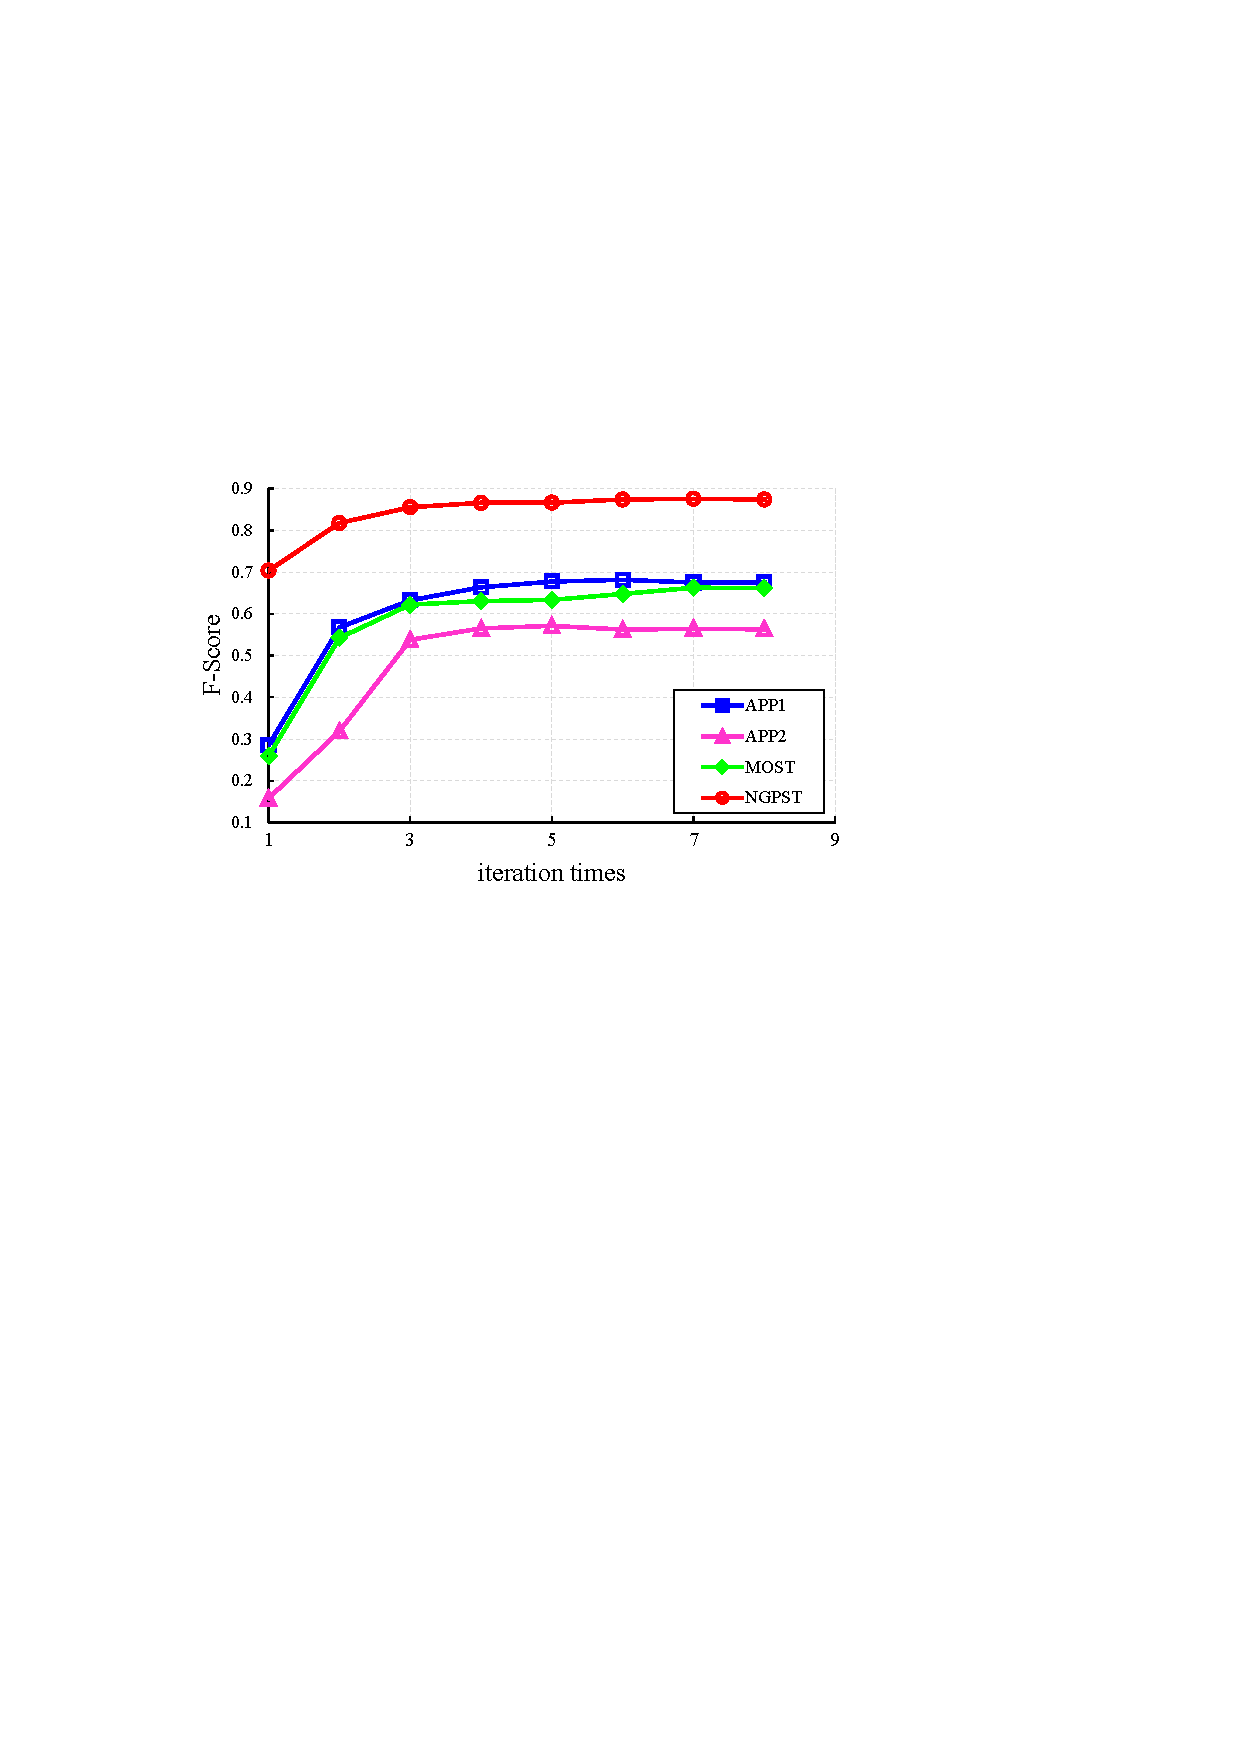
\includegraphics[width=0.8\columnwidth]{./Illustrations/trace_iterations_fscore8.pdf}
	\caption{Progressively improved F-score of neuron reconstruction results under eight iterations in our progressive learning framework using four neuron tracing methods.}% APP1~\cite{Peng2011} and its variant APP2~\cite{Xiao2013}, MOST\cite{Wu2014} and NGPST~\cite{Quan2015} on the VISoR-40 test dataset at eight iterations. For each of the four neuron tracing methods, our approach progressively improves their reconstruction results.} 
	\label{fig:fscore_iterations}
\end{figure}

\begin{figure*}[t]
	\centering
	\subfigure[]{
		\begin{minipage}[b]{0.32\linewidth}
			\centering
			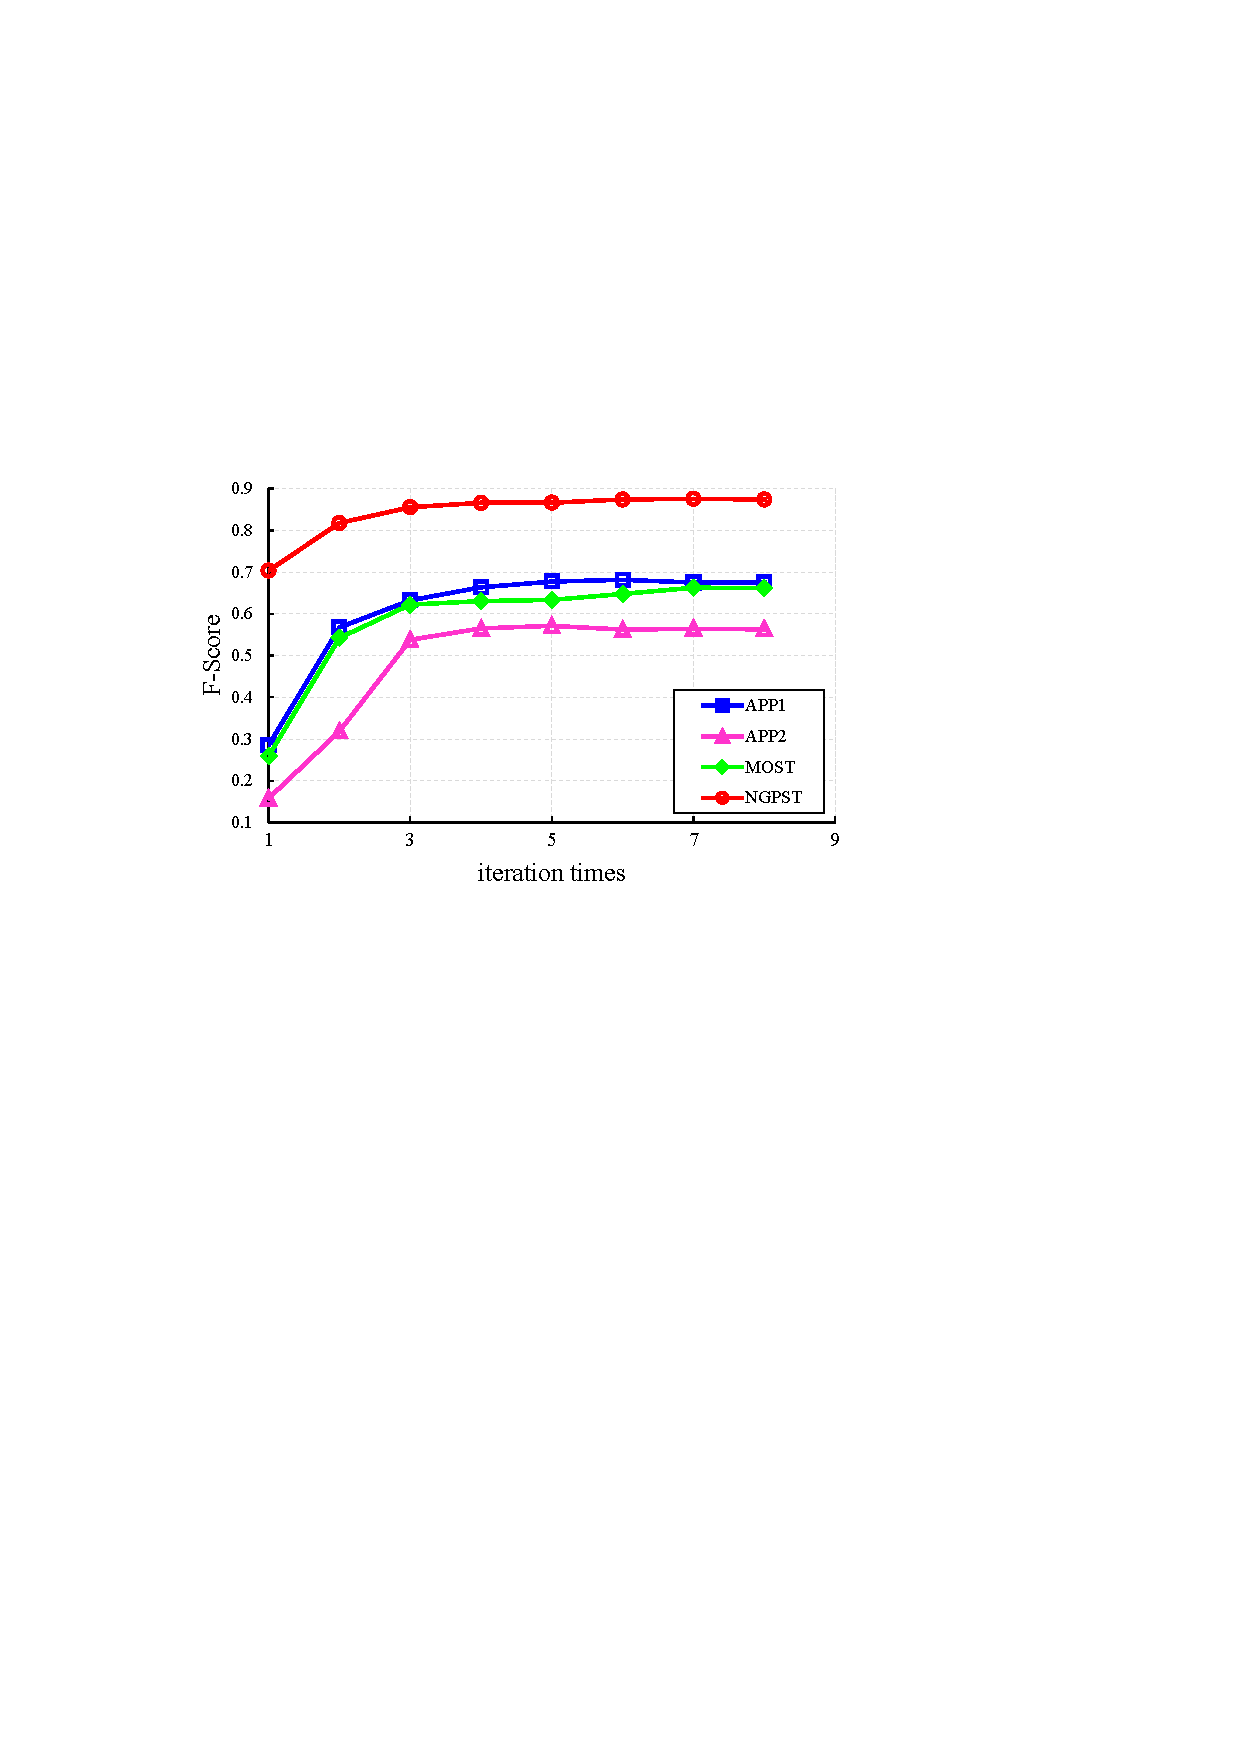
\includegraphics[height=3.7cm]{./Illustrations/trace_iterations_fscore8.pdf}
		\end{minipage}
	}
	%\hspace{0.1cm}
	\subfigure[]{
		\begin{minipage}[b]{0.32\linewidth}
			\centering
			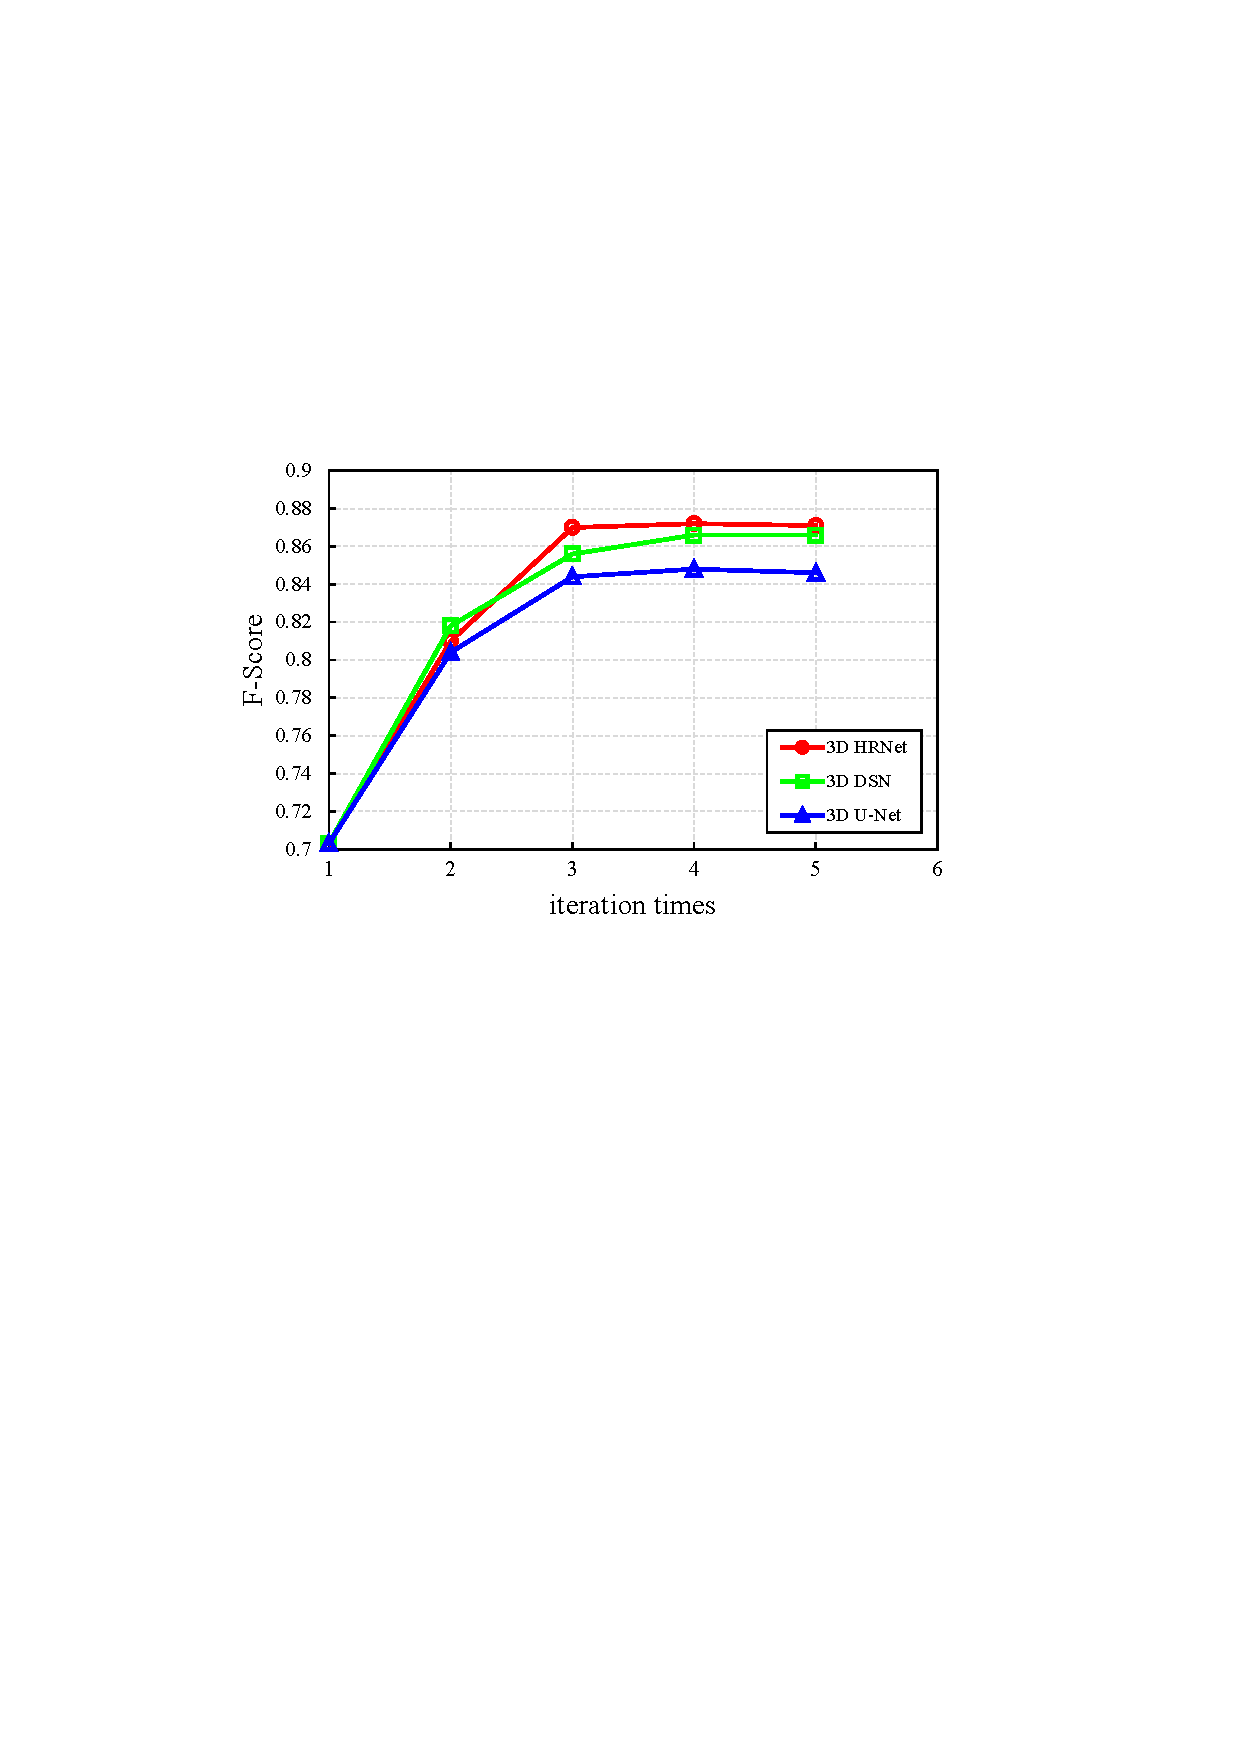
\includegraphics[height=3.7cm]{./Illustrations/trace_networks_fscore11.pdf}
		\end{minipage}
	}
	%\hspace{0.1cm}
	\subfigure[]{
		\begin{minipage}[b]{0.32\linewidth}
			\centering
			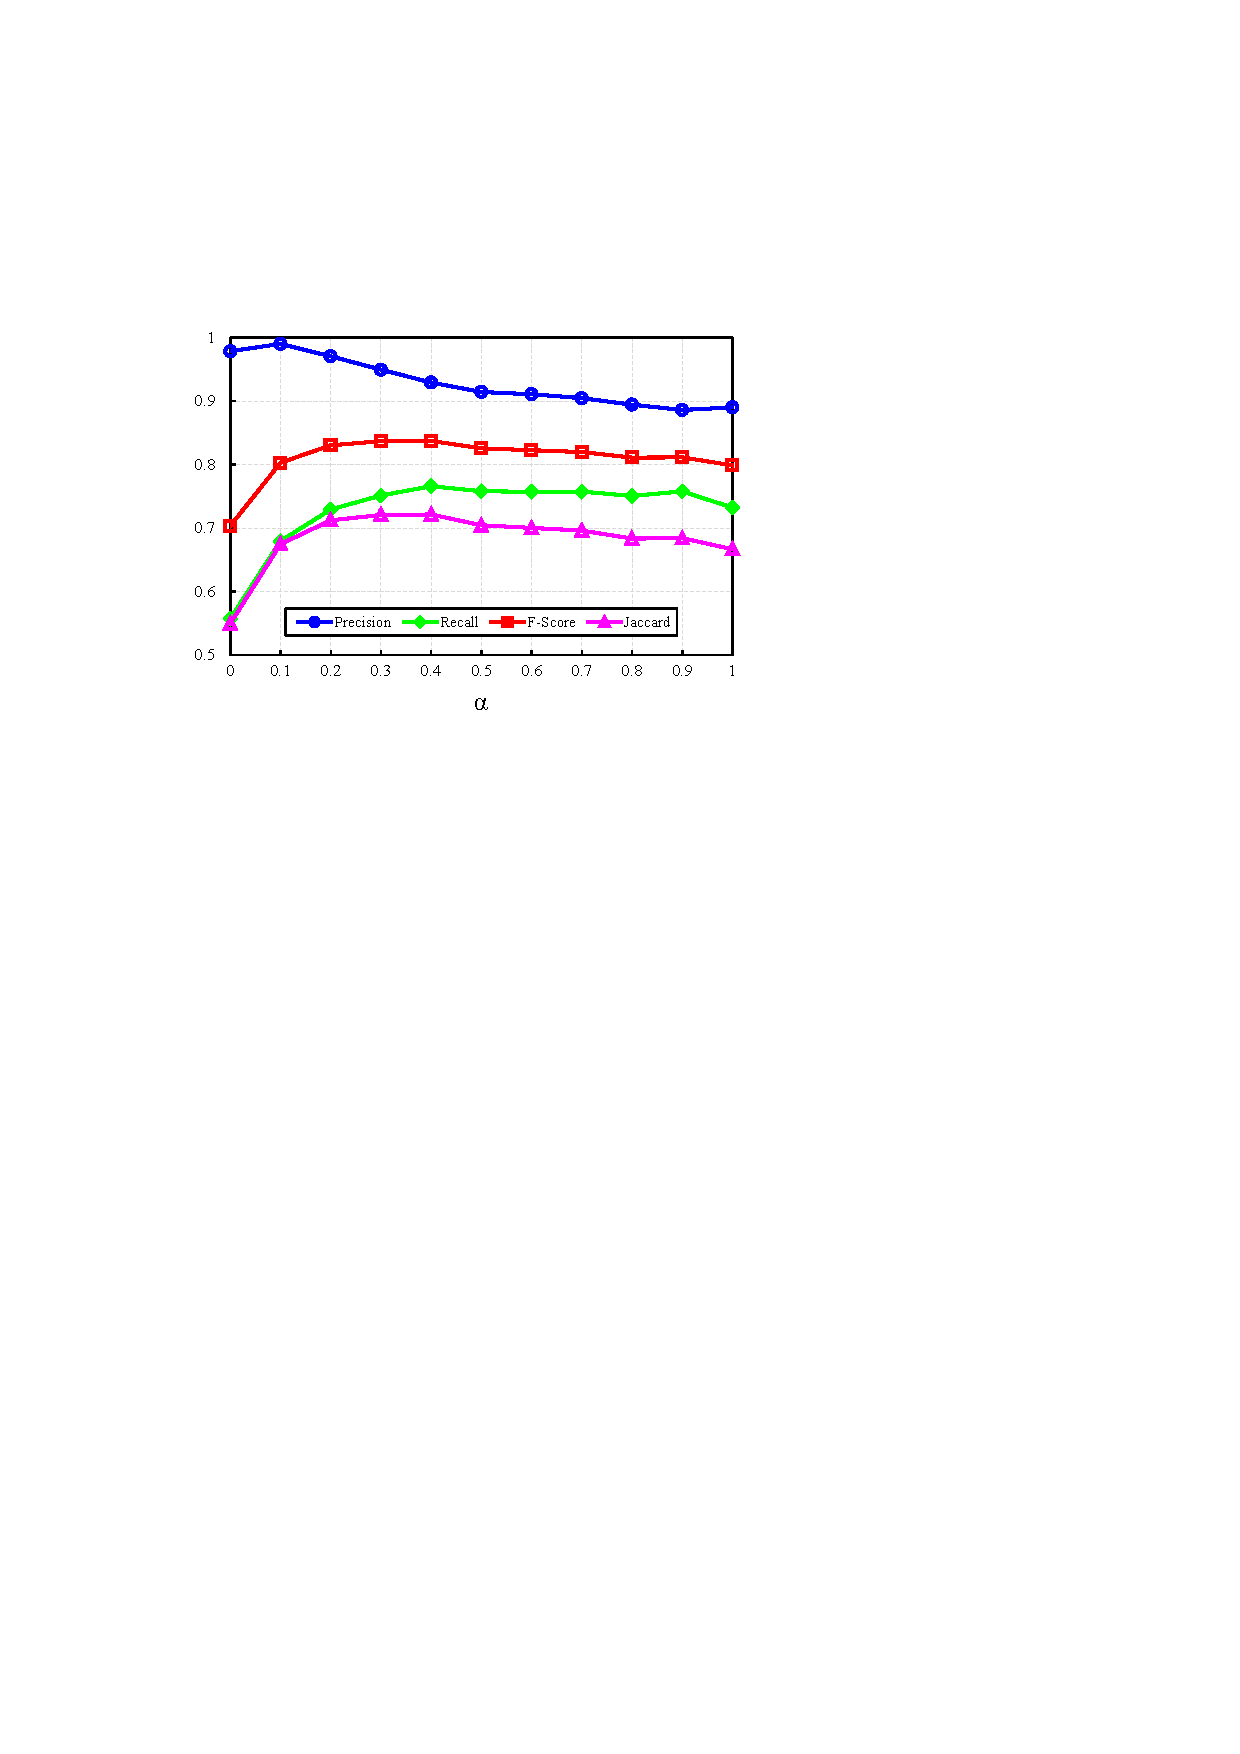
\includegraphics[height=3.7cm]{./Illustrations/weight_paprameter7.pdf}
		\end{minipage}
	}
	\caption{
	(a) Comparisons of neuronal population reconstruction performance on the VISoR-40 test dataset at different iterations using four neuron tracing methods.
	(b) F-Score of neuron reconstruction on the VISoR-40 testing dataset at five iterations. Combining any one of the three neuron segmentation networks, our approach progressively improves the reconstruction performance.
	(c) Neuron reconstruction performance with different $\alpha$ in Eq.~\eqref{equ: enhance} for image enhancement on the VISoR-40 test dataset. From left to right, the value of $\alpha$ increases from $0$ to $1$ by a step of $0.1$.}
	\label{fig:tracing_performance_plnpr}
\end{figure*}


\begin{figure}[t]
	\centering
	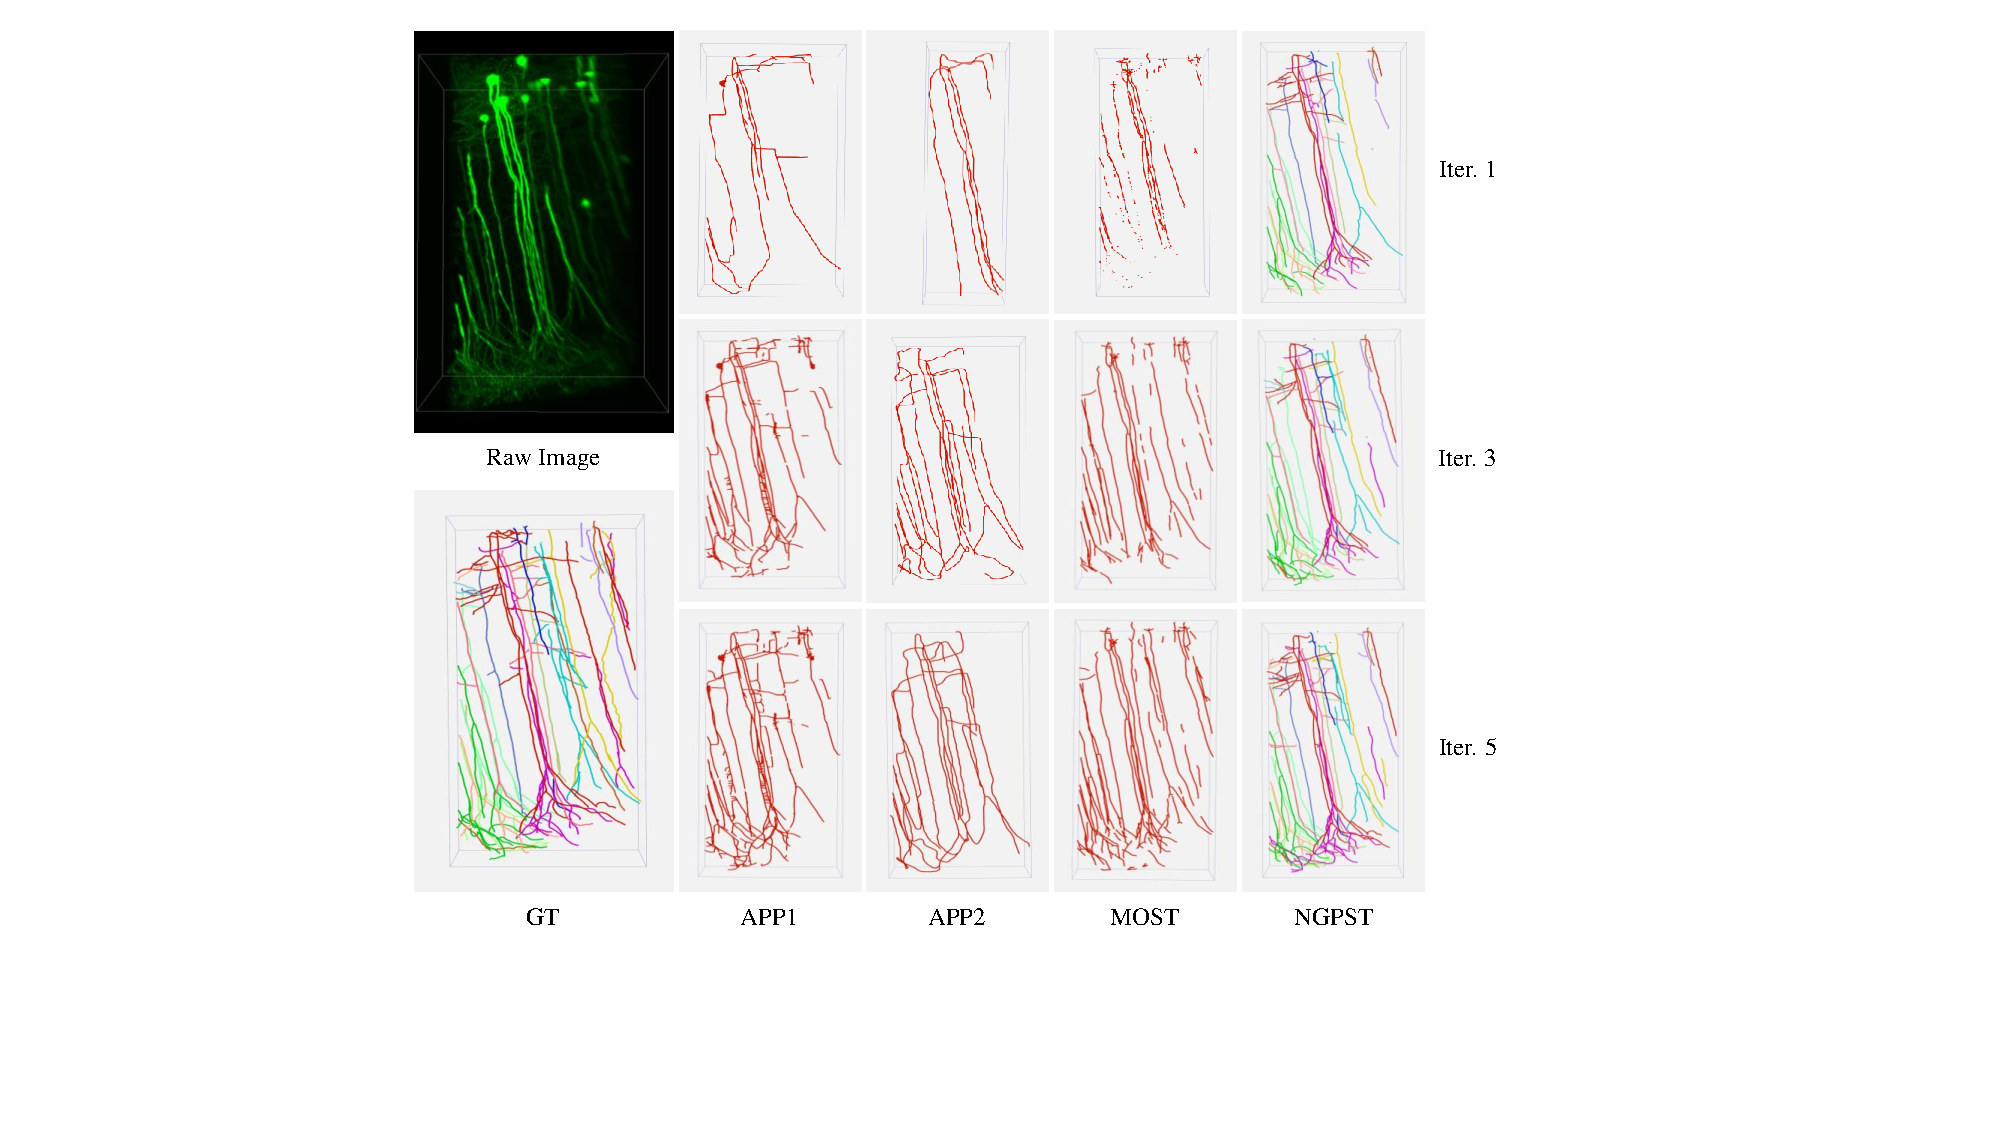
\includegraphics[width=1\columnwidth]{./Illustrations/trace_iterations3.pdf}
	\caption{Neuronal population reconstruction results of a test block at different iterations (top to bottom) using four neuron tracing methods.} 
	% APP1~\cite{Peng2011}, APP2~\cite{Xiao2013}, MOST\cite{Wu2014} and NGPST~\cite{Quan2015}.}
	\label{fig:trace_iterations}
\end{figure}

\begin{table}[t]
	\centering
	\caption{F-Score of neuron reconstruction on a test image block from the VISoR-40 dataset at different iterations.% using four neuron tracing methods APP1~\cite{Peng2011}, APP2~\cite{Xiao2013}, MOST\cite{Wu2014} and NGPST~\cite{Quan2015}.
	}
	\label{table:trace_iterations}
	\begin{tabular}{lccc}
		\toprule
		Method & iter-1 & iter-3 & iter-5\\
		\midrule
		APP1~\cite{Peng2011}
		& 0.315 & 0.599 & 0.599\\
		APP2~\cite{Xiao2013}
		& 0.251 & 0.511 & 0.538\\
		MOST~\cite{Wu2014}          
		& 0.322 & 0.588 & 0.721\\
		NGPST~\cite{Quan2015}
		& 0.758 & 0.825 & 0.888\\
		\bottomrule
	\end{tabular}
\end{table}

\begin{figure}[t]
	\centering
	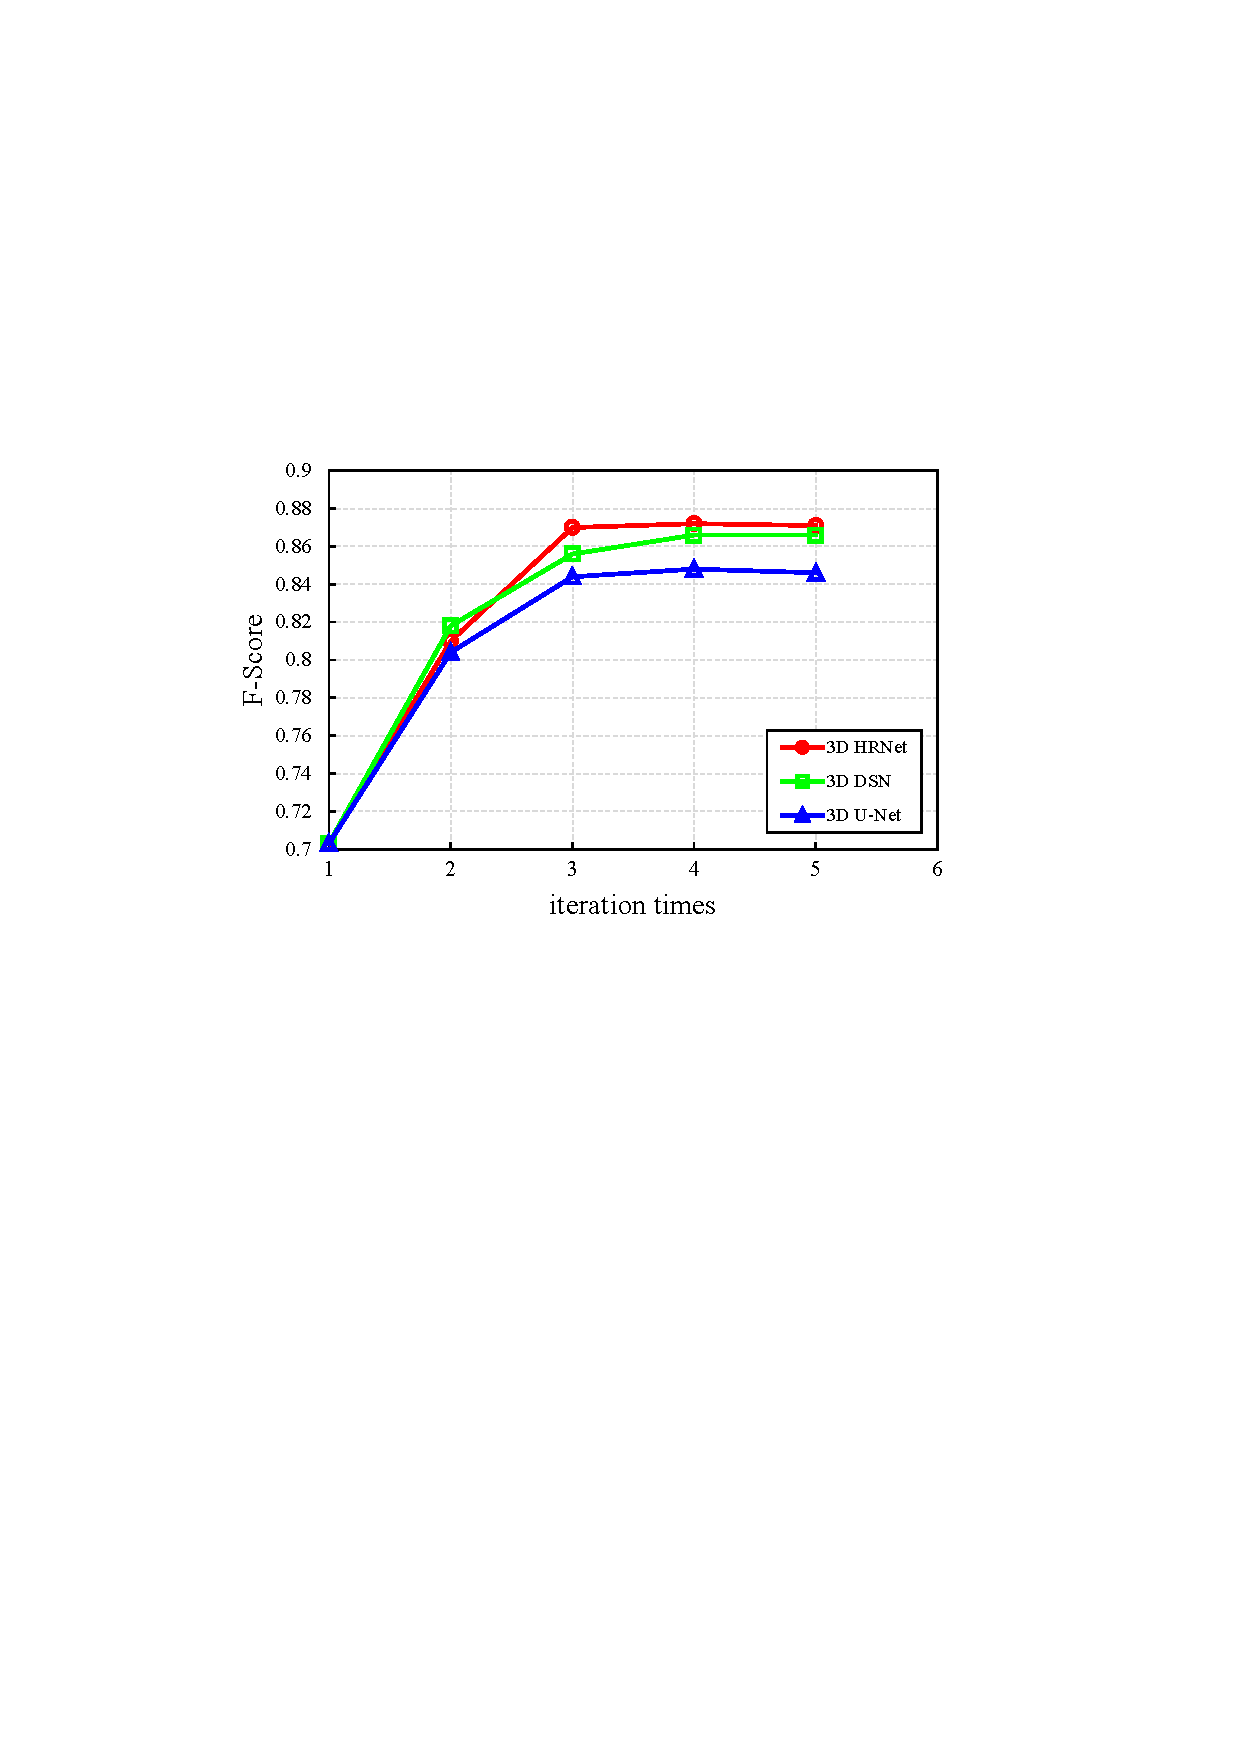
\includegraphics[width=0.8\columnwidth]{./Illustrations/trace_networks_fscore11.pdf}
	\caption{F-Score of neuron reconstruction on the VISoR-40 testing dataset at five iterations. Combining any one of the three neuron segmentation networks, our approach progressively improves the reconstruction performance.}
	\label{fig:fscore_DNNs}
\end{figure}



\subsubsection{Neuron Segmentation Network}

To further verify the effectiveness and robustness of our progressive learning strategy, we test three commonly used deep segmentation networks, including 3D DSN~\cite{Dou2017}, 3D U-Net~\cite{Cicek2016} and a 3D version of HRNet~\cite{Sun2019}, for generating the neuron probability map.
%All of them have the same input size, i.e. $160 \times 160\times 160$.
Five iterations are tested on our VISoR-40 dataset, and the F-Score improvement of reconstruction results is shown in the Fig.~\ref{fig:fscore_DNNs}. 
%
It can be seen that our PLNPR algorithm effectively improves the neuron reconstruction performance by combining any one of the three neuron segmentation networks.
Consequently, the segmentation network and traditional tracing method can complement and promote each other, leading to more complete reconstruction.


\subsubsection{Enhancement Parameter} 

In order to explore the influence of parameter $\alpha$ in Eq.~\eqref{equ: enhance} for image enhancement, we adopt different values for $\alpha$, and the results are shown in Fig.~\ref{fig:weight_paprameter}.
$\alpha=0$ means that the raw image block is directly used as input for the tracing module.
$\alpha=1$ means that only the probability maps are used as input for neuron tracing. 
It indicates that the performance is improved by combing the probability map with the raw intensity, mainly because that the probability map reflects the long-range trajectory structures while the original intensity preserves signal details to some extent.
%Second, it can be observed our system is very robust to the parameter $\alpha$. 
%Hence, the chosen of the parameter $\alpha$ is not very demanding and the reconstruction performance can achieve significant improvement with any $\alpha >0$. 
In this paper, we empirically select $\alpha=0.1$ to reduce the influence of false positive predictions in probability maps due to the limited performance of the DNN model trained by pseudo labels and increase the robustness of the whole framework.

\begin{figure}[t]
	\centering
	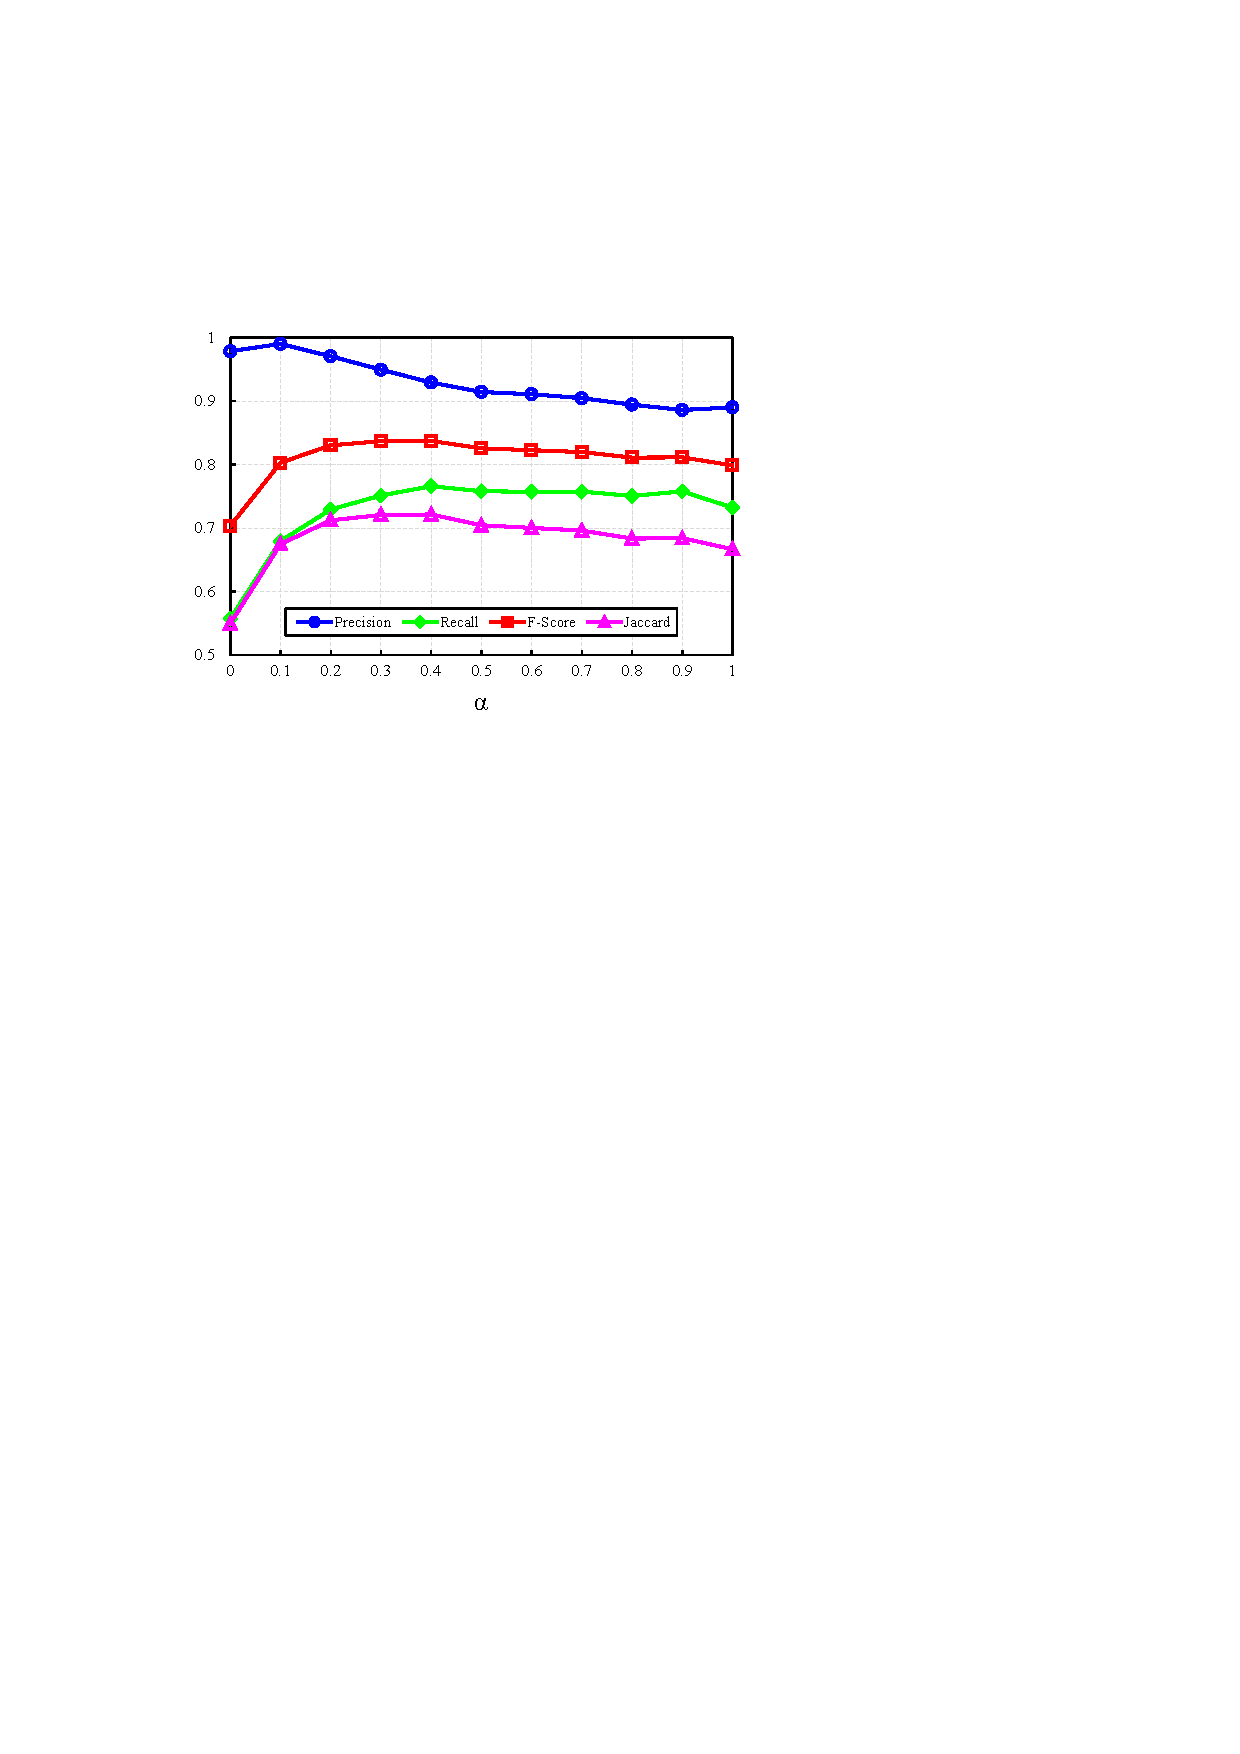
\includegraphics[width=0.8\columnwidth]{./Illustrations/weight_paprameter7.pdf}
	\caption{Neuron reconstruction performance with different $\alpha$ in Eq.~\eqref{equ: enhance} for image enhancement on the VISoR-40 test dataset. From left to right, the value of $\alpha$ increases from $0$ to $1$ by a step of $0.1$.  }
	\label{fig:weight_paprameter}
\end{figure}


\subsubsection{Comparison on VISoR-40 Dataset}



\begin{figure*}[t]
	\centering
	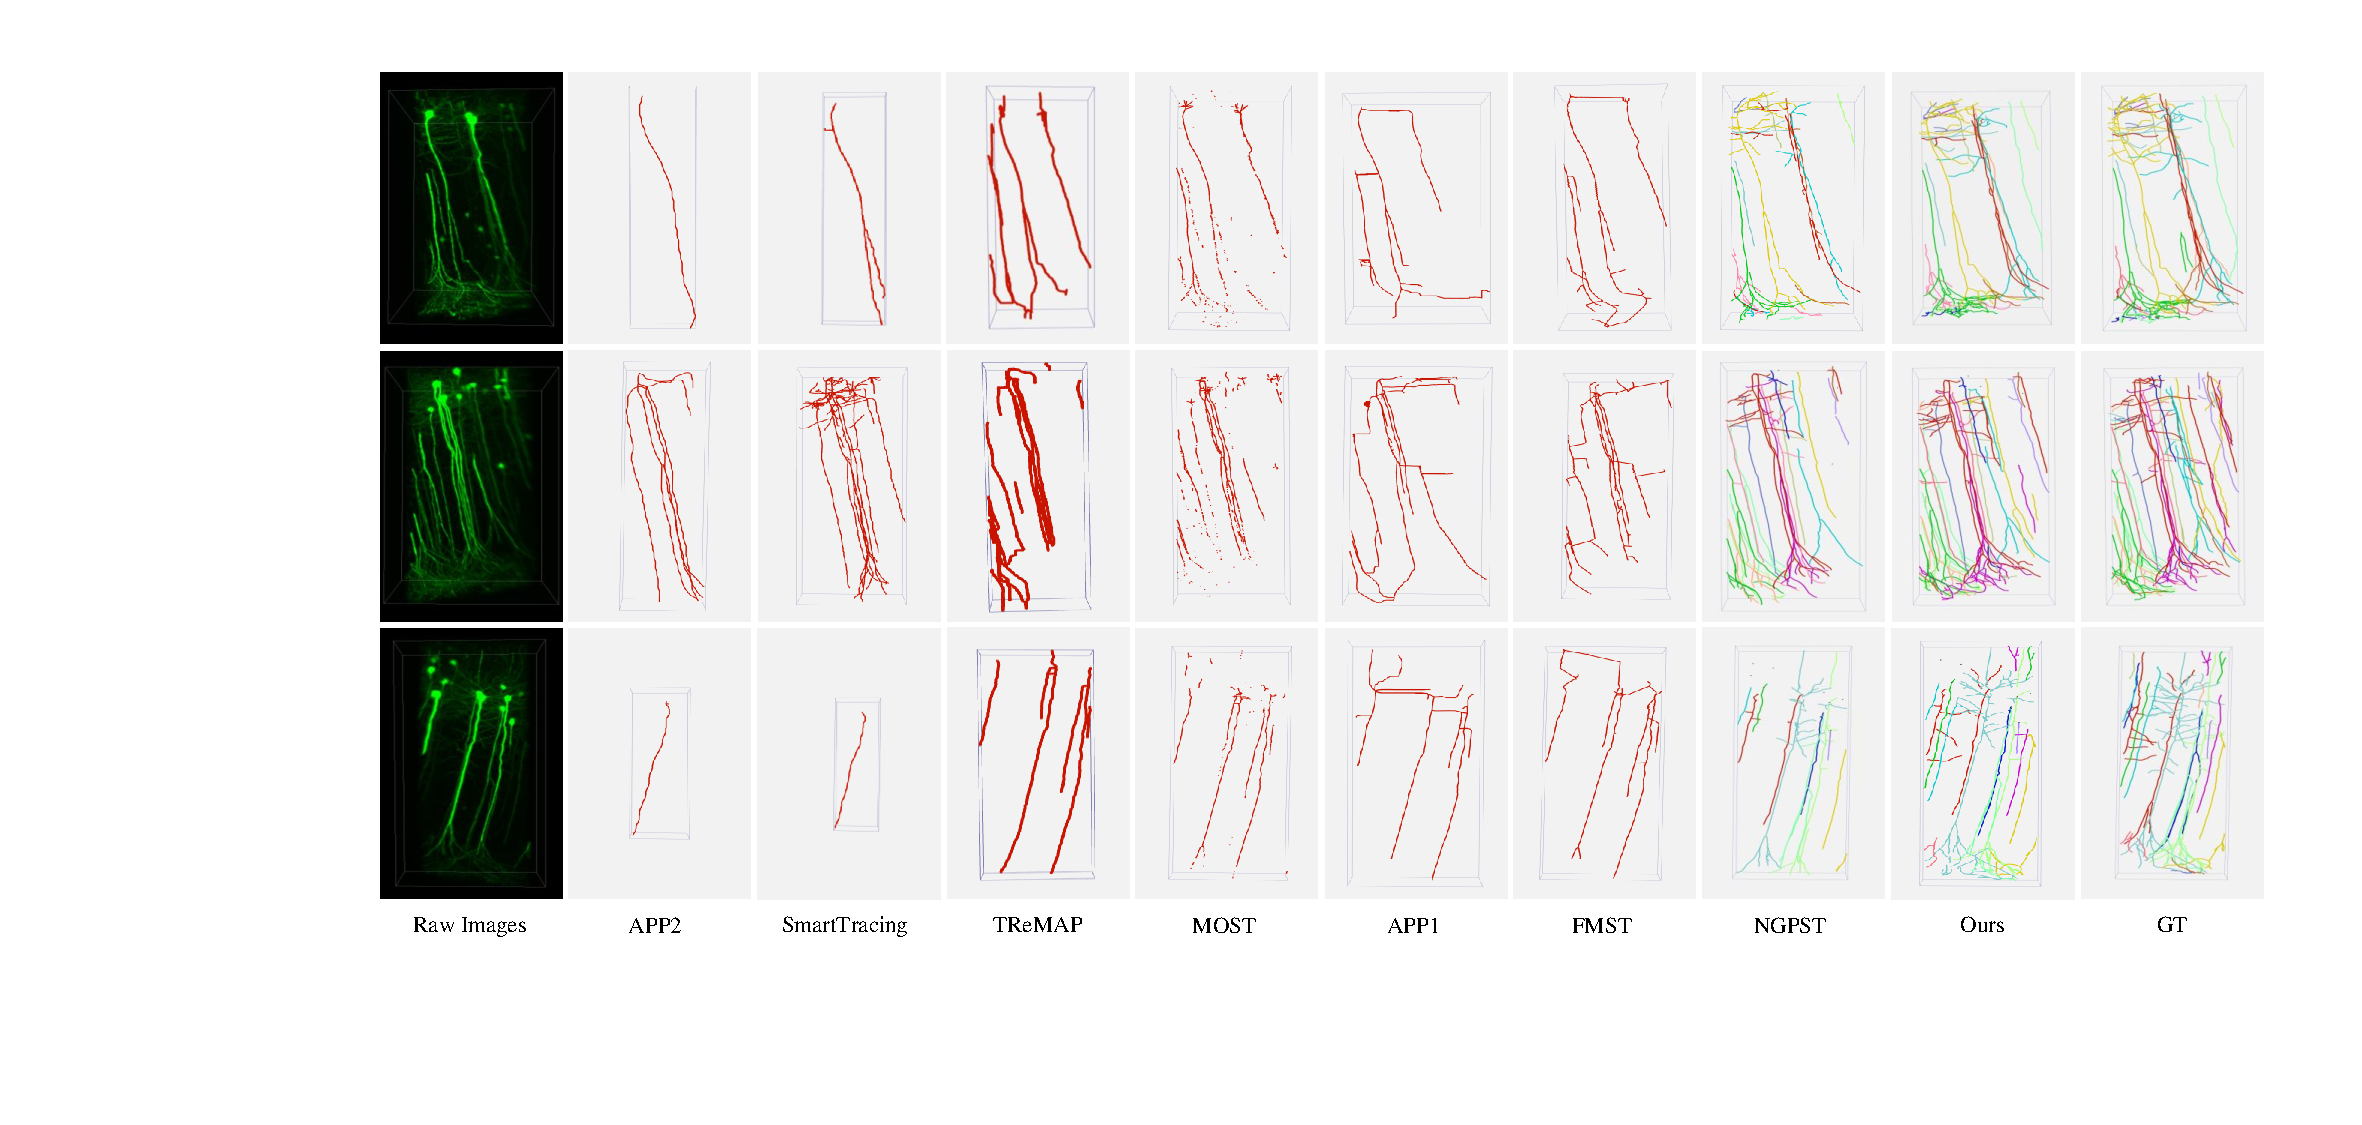
\includegraphics[width=1\textwidth]{./Illustrations/iteration3.pdf}
	\caption{Comparison of neuronal population reconstruction results of three image blocks. %using neuron reconstruction methods FMST~\cite{Yang2019}, APP1~\cite{Peng2011}, APP2~\cite{Xiao2013}, SmartTracing~\cite{Chen2015}, MOST~\cite{Wu2014}, NGPST~\cite{Quan2015} and our PLNPR on three test images from the VISoR-40 dataset.
%	Each row shows the reconstruction results generated by different methods for a test image. The first column shows the raw images, while the last column shows the ground truth (GT). Each of the remaining columns shows the reconstruction result using the corresponding tracing method. 
Our PLNPR method reconstructs more complete and accurate neurons compared to other methods. 
	}
	\label{fig:compare_VISoR}
\end{figure*}



\begin{table*}[th]
	\centering
	\caption{Performance comparison with different methods for neuronal population reconstruction on the VISoR-40 dataset.}
	\label{table:compare_VISoR}
	\begin{tabular}{lcccc}
		\toprule
		Method & Precision & Recall & F-Score & Jaccard\\
		\midrule
		%\hline
		APP2~\cite{Xiao2013}
		& \textbf{0.980} & 0.091 & 0.157 & 0.091\\
		SmartTracing~\cite{Chen2015}
		& 0.961 & 0.133 & 0.205 & 0.128\\
		TReMAP~\cite{Zhou2016}
		& 0.917 & 0.147 & 0.253 & 0.145\\
		MOST~\cite{Wu2014}          
		& 0.969 & 0.151& 0.258& 0.151\\
		APP1~\cite{Peng2011}
		& 0.935 & 0.169 & 0.284 & 0.167\\
		FMST~\cite{Yang2019}
		& 0.884 & 0.179 & 0.296 &  0.176\\
		NGPST~\cite{Quan2015}
		& 0.978 & 0.557& 0.703 & 0.549\\
		\midrule
		Ours
		& 0.971 & \textbf{0.801}&\textbf{0.875} & \textbf{0.781}\\
		\bottomrule
	\end{tabular}
\end{table*}

%<18-AAAI-Adaptive Graph Convolutional Neural Networks>
To prove the effectiveness of our method on neuronal population reconstruction, we compare it with seven widely used neuron tracing methods, including APP1~\cite{Peng2011},  APP2~\cite{Xiao2013}, MOST~\cite{Wu2014}, SmartTracing~\cite{Chen2015}, NGPST~\cite{Quan2015}, TReMAP~\cite{Zhou2016} and  FMST~\cite{Yang2019}.
\md{The parameters of these tracing methods are manually adjusted for each image to get optimal performance in the experiments.}
%
We utilize NGPST with 3D DSN enhancement as ``Ours''. \md{Note that the segmentation network in our approach is trained progressively on the VISoR-40 dataset in the training stage. We use the trained model directly at the testing stage for evaluation. }
%
Table~\ref{table:compare_VISoR} compares the quantitative results of different methods with regard to Precision, Recall, F-Score and Jaccard.
%
It shows that our method makes a significant improvement on the overall performance compared with other methods.
\md{Though APP2 achieves the highest precision, the reconstructed neurons are significantly sparser than others. }
\xj{What happens if you provide multiple somas for APP2? }
%
Fig.~\ref{fig:compare_VISoR} shows the neuronal populations reconstructed from three testing image blocks.
%
Compared with other methods, our PLNPR is superior in both sparse and dense neurons.
Conventional methods~\cite{Peng2011, Xiao2013, Wu2014, Zhou2016} and learning-based methods~\cite{Chen2015, Yang2019} tend to extract the main trunk of neurons, while missing a large portion of subtle neurites. 
Therefore, these methods have very high precision but significantly lower recall.
Although NGPST~\cite{Quan2015} achieves better performance of neuronal identity, it still remains difficult to extract subtle neuron voxels by using hand-crafted features.
%
In comparison, our method benefits from the progressively trained segmentation network, and reconstructs more complete neurons from challenging blocks, even there exhibit noises, low contrast and blending of fluorescence in the blocks.


\subsection{Evaluation of PLNPR on BigNeuron Dataset}
\label{sec:exp_PLNPR_BigNeuron}

\subsubsection{BigNeuron Dataset}

To validate our PLNPR method on single neuron reconstruction, we employ the BigNeuron~\cite{peng2015} dataset which is a well-known community-derived neuron dataset. 
This dataset totally consists of about $20,000$ 3D OM images, acquired from a variety of species and optical imaging systems.
%Some images have the corresponding manual annotations for evaluation.  
Unlike our VISoR-40 dataset which is built for the evaluation of neuronal population reconstruction, each block in the BigNeuron dataset contains a single neuron or fragmented neurites.
% which are appropriate for single neuron reconstruction.
\md{Following \cite{Li2017}, we select the same 68 images that are from a variety of species.
Manual reconstruction by experts is associated with each image. 
51 images are used for network training and the remaining 17 images are used for evaluation.}


\subsubsection{Experimental Settings and Evaluation Metrics}
 
\md{
To evaluate our PLNPR on the single neuron reconstruction, we use the DSN model pretrained on the VISoR-40 dataset as initialization and fine-tune it on the BigNeuron dataset using pseudo labels generated by NGPST~\cite{Quan2015} instead of the provided manual annotations.
%
The learning rate was initialized as $\num{1e-4}$ and decayed using the ``poly" learning rate policy (power of $0.9$). The maximum iteration number is set to $ 24000 $.
We cropped patches of size $160\times 160\times 8$ as input to the network, considering consumption of the GPU memory, and also unequal image sizes along three directions.
}
\xj{Do you use 160x160x160 on the Visor-40 dataset?}

\md{
Since the implementation of most learning-based tracing methods, such as~\cite{Li2017} are not publicly available, to compare with~\cite{Li2017}, the testing data and three evaluation metrics for evaluation are the same as those used in~\cite{Li2017}.
The three measurements defined in~\cite{Peng2010a} include entire structure average (ESA), different structure average (DSA) and percentage of different structures (PDS). For all of these three scores, larger values indicate higher discrepancy between the tracing results and the manual reconstruction.
}
 


\subsubsection{Comparison on BigNeuron Dataset}

\begin{figure*}[th]
	\centering
	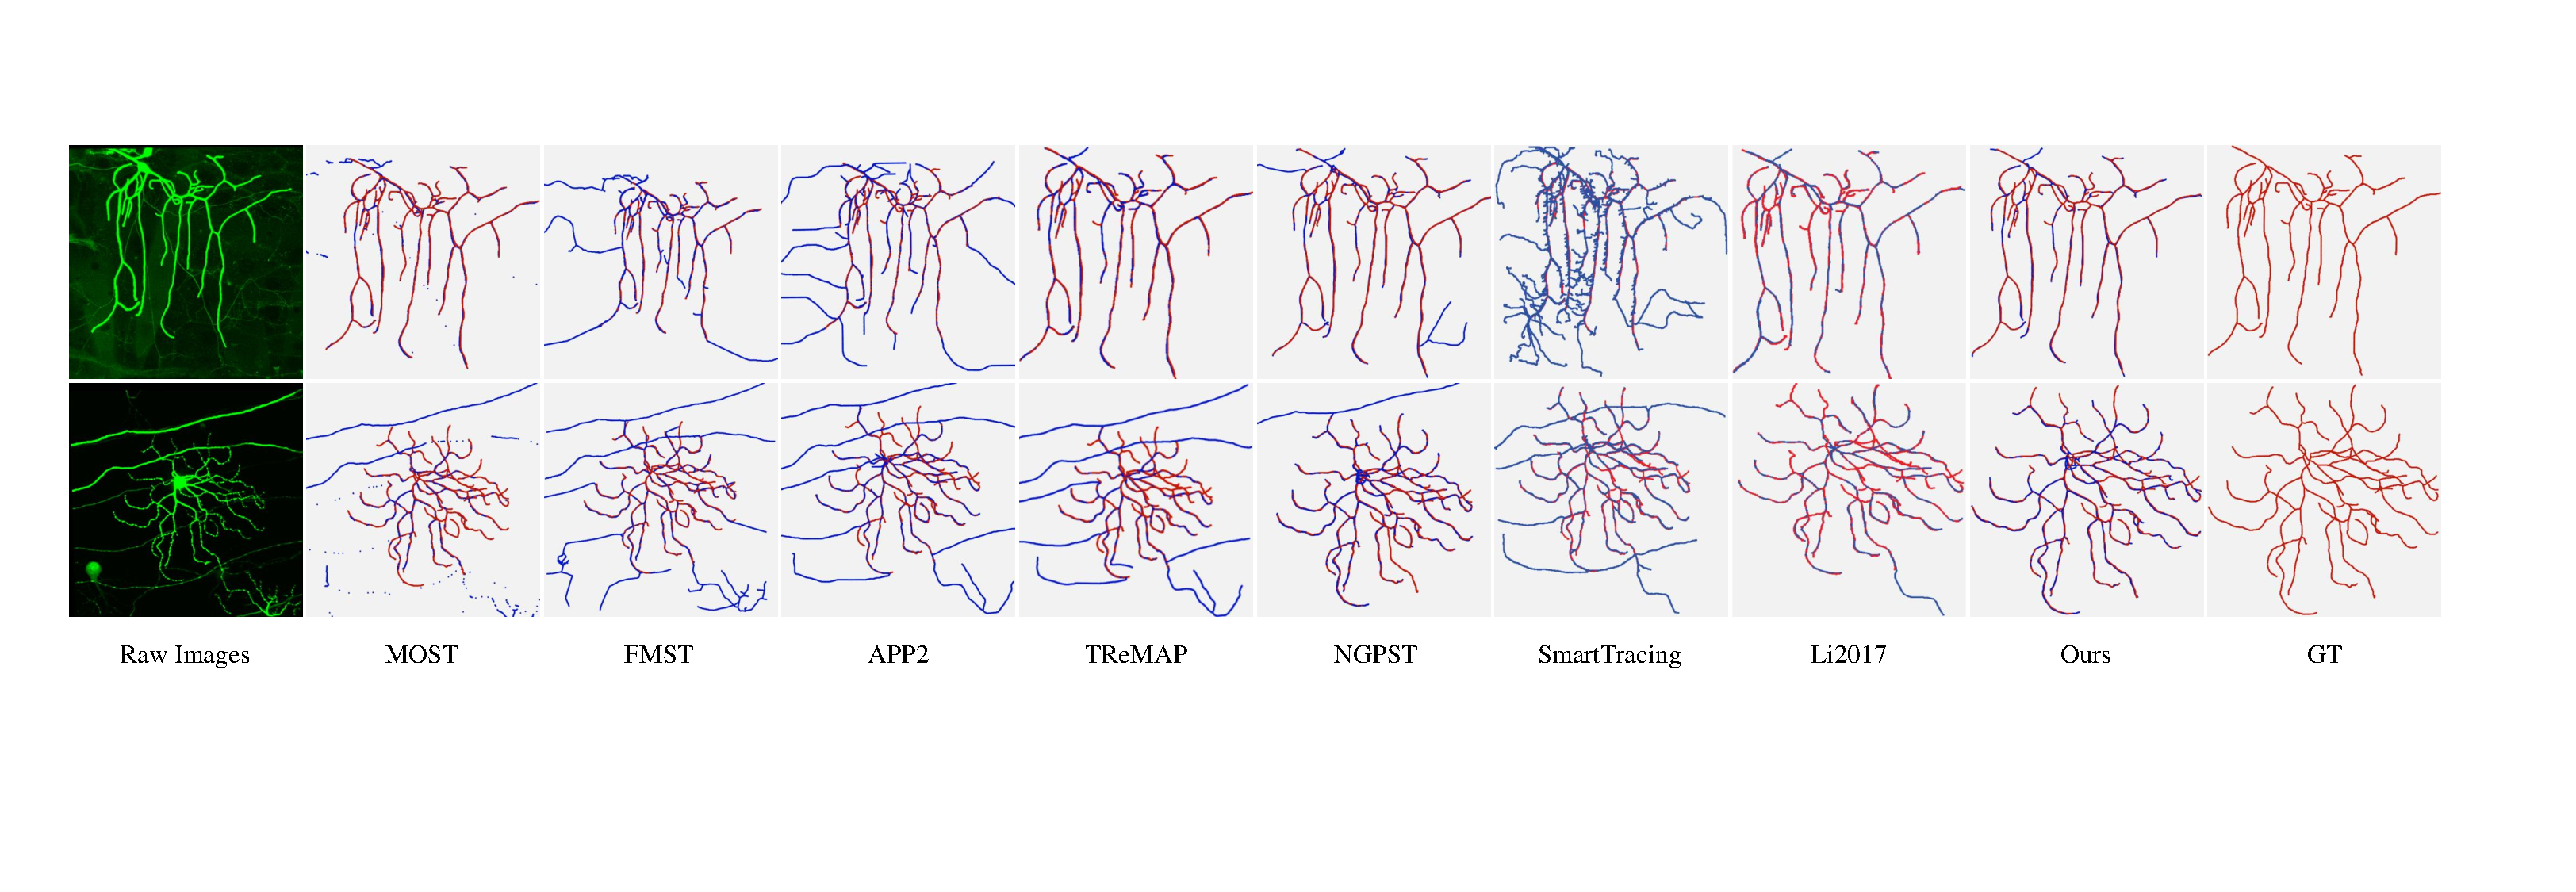
\includegraphics[width=1\textwidth]{./Illustrations/BigNeuron6.pdf}
	\caption{Comparison of single neuron reconstruction results on two test images from the BigNeuron dataset.
		% using MOST~\cite{Wu2014}, FMST~\cite{Yang2019}, APP2~\cite{Xiao2013}, TReMAP~\cite{Zhou2016}, NGPST~\cite{Quan2015}, SmartTracing~\cite{Chen2015}, Li2017~\cite{Li2017} and our PLNPR on two testing images from the BigNeuron dataset.
	%Each row shows the reconstruction results generated by different methods for a test image. The first column shows the raw images, while the last column shows the ground truth (GT). Each of the remaining columns shows the reconstruction result using the corresponding tracing method. 
	The reconstruction neurites are shown in blue and the corresponding ground truth (GT) are shown in red.
	Our method reconstructs more complete and accurate neurons compared to other methods.
	}
	\label{fig:compare_BigNeuron}
\end{figure*}

\begin{table*}[th]
	\centering
	\makeatletter\def\@captype{table}\makeatother
	\caption{Performance comparison for single neuron reconstruction on the BigNeuron test dataset.}
	\label{table:compare_BigNeuron}
	\begin{tabular}{lccccccc}
		\toprule
		Method & Precision & Recall & F-Score & Jaccard & ESA & DSA & PDS\\
		\midrule
		MOST~\cite{Wu2014} & 0.619 & 0.361 & 0.456 & 0.295 & 31.730 & 38.211 & 0.633\\
		FMST~\cite{Yang2019} & 0.575 & 0.629 & 0.601 & 0.429 & 17.878 & 23.459 & 0.558\\
		APP2~\cite{Xiao2013} & \textbf{0.799} & 0.492 & 0.608 & 0.437 & 13.457 & 17.923 & 0.562\\
		TReMAP~\cite{Zhou2016} & 0.771 & 0.415 & 0.539 & 0.369 & 11.269 & 17.941 & 0.539\\
		NGPST~\cite{Quan2015} & 0.710 & 0.680 & 0.695 & 0.532 & 10.168 & 14.880 & 0.587\\
		SmartTracing~\cite{Chen2015} & 0.701 & 0.648 & 0.674 & 0.508 & 8.532 & 11.609 & 0.543\\
		Li2017~\cite{Li2017} & - & - & - & - & 4.917 & \textbf{7.972} &0.461 \\
		\midrule
		Ours & 0.790 & \textbf{0.707} & \textbf{0.746}  & \textbf{0.595} & \textbf{4.784} & 8.309 & \textbf{0.451}\\
		\bottomrule
	\end{tabular}
\end{table*}

\begin{figure}[t]
	\centering
	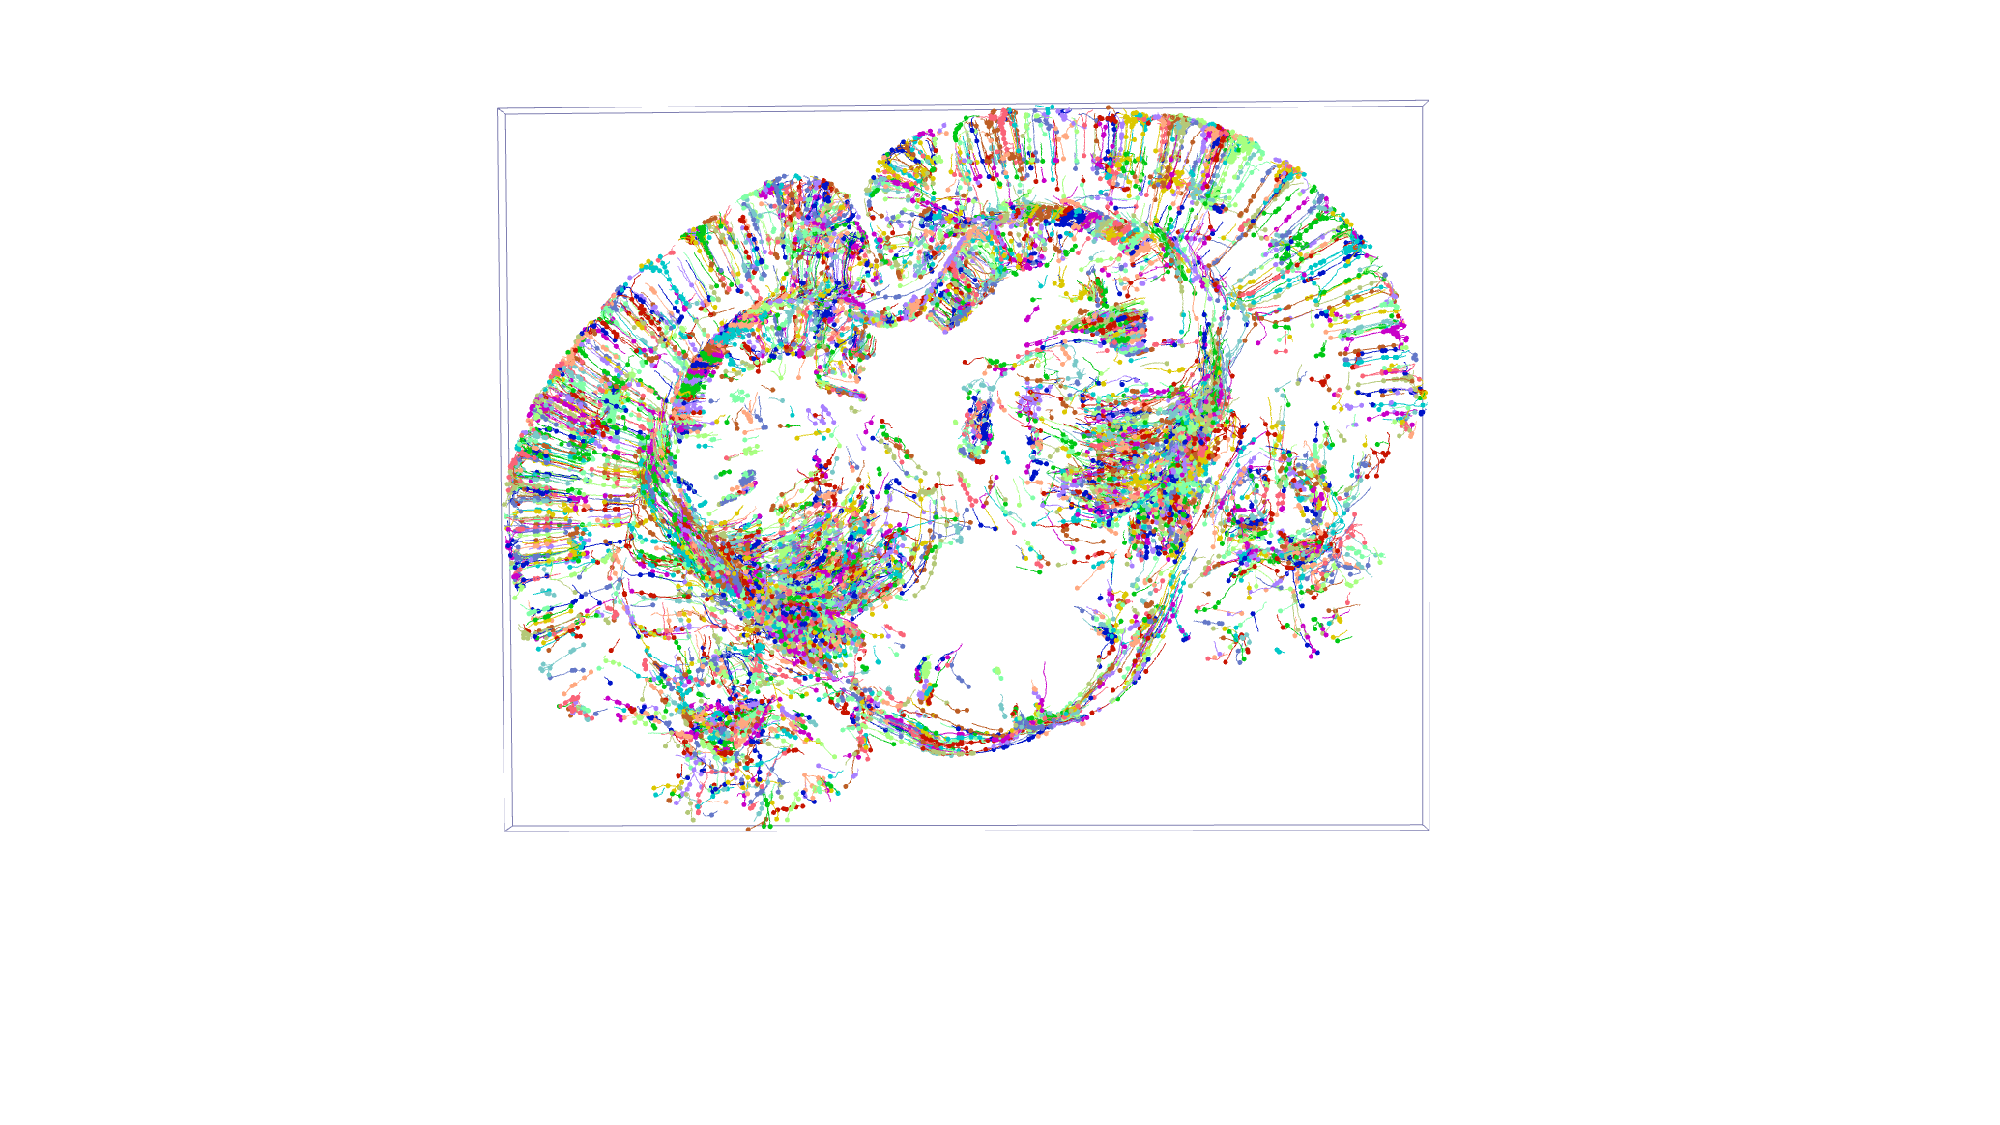
\includegraphics[width=1\columnwidth]{./Illustrations/brain_slice.pdf}
	\caption{The reconstruction result of neuronal populations in a large-scale 3D mouse brain slice using our UltraNPR method.}
	\label{fig:reconstruct_brain}
\end{figure}


On the BigNeuron dataset, we compare with seven widely used tracing methods to validate the effectiveness of our proposed method.
They are APP2~\cite{Xiao2013}, MOST~\cite{Wu2014}, SmartTracing~\cite{Chen2015}, NGPST~\cite{Quan2015}, Li2017~\cite{Li2017}, TReMAP~\cite{Zhou2016} and FMST~\cite{Yang2019} respectively.
%To compare with the deep learning based method, the testing data and three evaluation metrics for evaluation are the same as those used in~\cite{Li2017}. The three measurements include different structure average (DSA), percentage of different structures (PDS) and entire structure average (ESA).
Fig.~\ref{fig:compare_BigNeuron} visualizes the neurons reconstructed from two testing blocks.
%``Ours'' means that we utilize NGPST with DSN, which is progressively trained on the VISoR-40 dataset first and then fine-tuned on the BigNeuron dataset using pseudo labels instead of the provided manual annotations.
%It can be seen that
Our method reconstructs more accurate neuronal morphology compared with other methods.
%The weighted average of the ESA, DSA and PDS on all testing images are listed in Table~\ref{table:compare_BigNeuron}.
In Table~\ref{table:compare_BigNeuron}, we list the weighted average of the DSA, PDS and ESA on all testing data using different methods.
%The weights are proportional to the neuron lengths identified in manual annotations.
The weight of each testing block is proportional to the neuron length identified in the corresponding manual annotation.
From Table~\ref{table:compare_BigNeuron}, we can observe that our method outperforms others in both PDS and ESA metrics and also achieves comparable performance in DSA metric with the best one.
In particular, unlike~\cite{Li2017} requiring on a strongly supervised network, our method obtains even better performance without any manual annotations.
With ever-increasing number of unlabeled neuron datasets are collected, our method can easily utilize them to further improve the performance of neuron reconstruction.

%\delete{To further validate the effectiveness of our PLNPR method, we also compare our results with seven methods on the BigNeuron~\cite{peng2015} dataset, including MOST~\cite{Wu2014}, FMST~\cite{Yang2019}, APP2~\cite{Xiao2013}, TReMAP~\cite{Zhou2016}, NGPST~\cite{Quan2015}, SmartTracing~\cite{Chen2015} and Li2017~\cite{Li2017}. For a fair comparison with deep learning based method, we use the testing data and three evaluation metrics the same as~\cite{Li2017}. Specifically, these metrics are entire structure average (ESA), different structure average (DSA) and percentage of different structures (PDS). Fig.~\ref{fig:compare_BigNeuron} shows the reconstruction results using different methods on two test images. The weighted average of the ESA, DSA and PDS on all test images of different methods are reported in Table~\ref{table:compare_BigNeuron}. The weights are proportional to the neuron lengths identified in the ground truth. ``Ours" means that we use NGPST with DSN enhancement after progressive learning on the VISoR-40 dataset first and then finetuned on BigNeuron dataset using pseudo labels rather than using the provided annotations. It can be seen that our method outperforms others in both ESA and PDS metrics and also achieves comparable performance in DSA metric with the best one. In particular, different from the supervised deep learning based method~\cite{Li2017}, our PLNPR gets even better performance without using any manual annotations. With ever increasing amounts of unlabeled microscopic datasets are collected, our method can easily utilize these datasets to further improve the performance of neuron reconstruction.}

\subsection{Evaluation of UltraNPR on a Mouse Brain Slice}
\label{sec:exp_UltraNPR}

%\subsubsection{Experimental Settings}
To reconstruct dense neuron populations in an ultra-scale image, we divide the entire image into blocks in size of $1120\times 2048\times 869$ considering the memory and computational efficiency of our PLNPR.
The overlap between adjacent blocks is set to be $300$ voxels along each dimension. 
The $\delta_{ovlp}$ is set to be 10 voxels.
The $\delta_{\alpha}$ is set to be 70 voxels and the $\beta$ is set to be 10 voxels.
%
Our UltraNPR takes just over one day \xj{in hours} to reconstruct the image on a cluster computer with $64$ GB of working memory and 20 NVIDIA 1080Ti GPUs.
%
As shown in Fig.~\ref{fig:reconstruct_brain}, a neuronal population which consists of $5348$ neurons is successfully reconstructed from the large-scale image.



\begin{figure}[t]
	\centering
	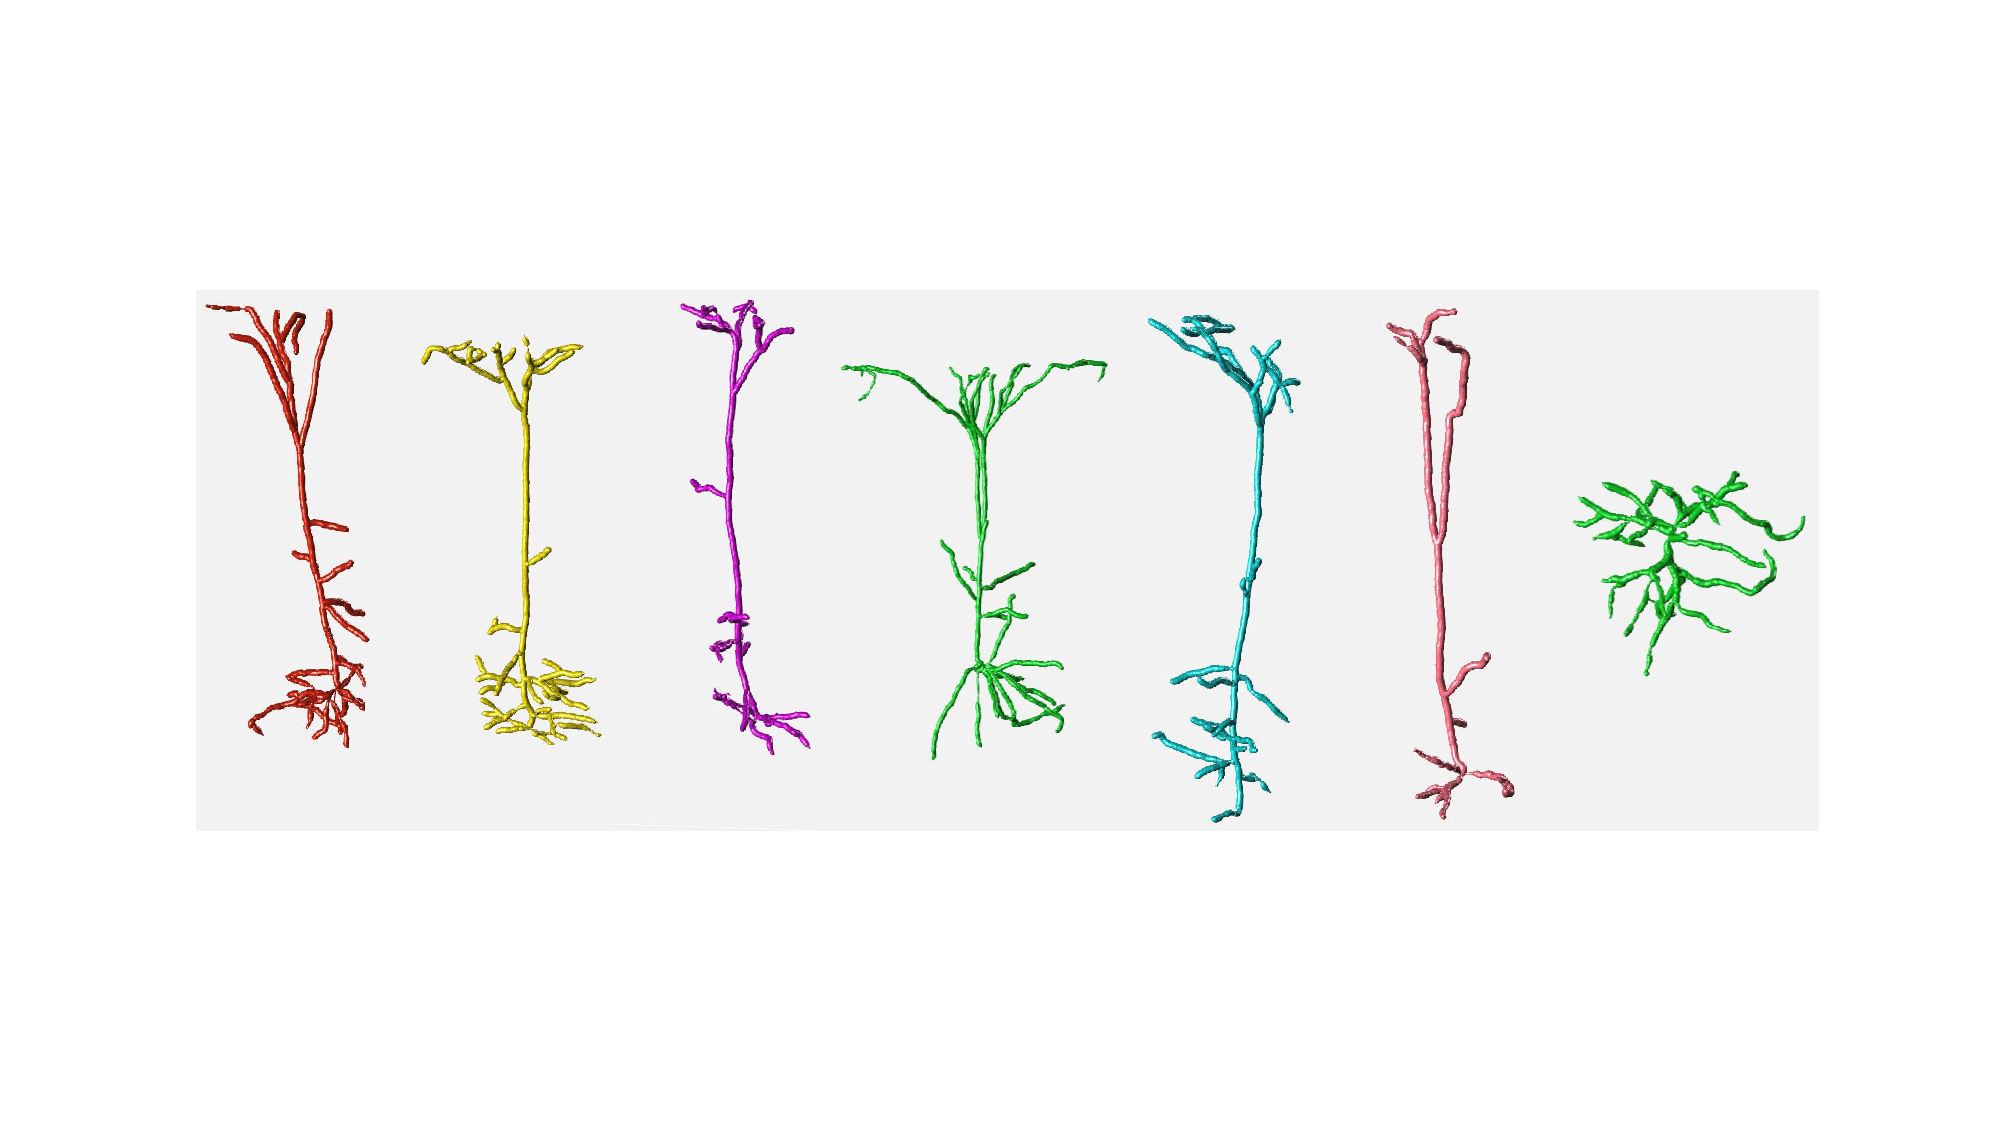
\includegraphics[width=0.8\columnwidth]{./Illustrations/single_neurons4.pdf}
	\caption{Single neurons selected from the reconstructed neuronal populations in a mouse brain slice using our UltraNPR method.}
	\label{fig:single_neurons}
\end{figure}


Several neurons selected from the reconstructed neuronal population are visualized in Fig.~\ref{fig:single_neurons}. These reconstructions provide detailed neuronal structures and enable further neuronal morphology analysis. 
In summary, our UltraNPR is capable of reconstructing dense neuronal populations from noisy and large-scale OM brain images.

Neuron length, number of branches.

\md{Since the manual annotation of neuronal populations from noisy OM images is difficult to obtain, let along the annotation of large-scale neuronal populations from a mouse brain slice. In this section, some qualitative results are visualized for verifying the effectiveness of our UltraNPR method.}